\documentclass[aspectratio=169]{beamer}

\usepackage{xcolor}
\usepackage{tikz}
\usepackage{stackrel}
\usepackage{bm,bbm}% bold math
\usepackage[version=3]{mhchem}
\usepackage{lmodern}

\usepackage{multirow}
\usepackage{setspace}
\usepackage{yfonts}
\usepackage{mathrsfs}
\usepackage{tcolorbox}
\usepackage{colortbl}
\usepackage{commath}
\usepackage{empheq}
\usepackage{multicol}
\usepackage{mhchem}

% Support for Pandoc-beamer
\usepackage[T1]{fontenc}
\usepackage{booktabs}
\usepackage{longtable}
\usepackage{fancyvrb}
\providecommand{\tightlist}{%
  \setlength{\itemsep}{0pt}\setlength{\parskip}{0pt}}

\usepackage[retainorgcmds]{IEEEtrantools}
\usepackage{siunitx}     
\sisetup{detect-display-math=true,detect-weight=true,detect-family=true}

\usepackage{tcolorbox,xcolor,framed}
\DefineVerbatimEnvironment{Highlighting}{Verbatim}{fontsize=\footnotesize,commandchars=\\\{\}}
\definecolor{shadecolor}{rgb}{0.9,0.9,0.9}
\newenvironment{Shaded}{\snugshade}{\endsnugshade}
\newcommand{\KeywordTok}[1]{\textcolor[rgb]{0.13,0.29,0.53}{\textbf{#1}}}
\newcommand{\DataTypeTok}[1]{\textcolor[rgb]{0.13,0.29,0.53}{#1}}
\newcommand{\NormalTok}[1]{#1}
\newcommand{\DecValTok}[1]{\textcolor[rgb]{0.00,0.00,0.81}{#1}}
\newcommand{\CommentTok}[1]{\textcolor[rgb]{0.56,0.35,0.01}{\textit{{#1}}}}
\newcommand{\PreprocessorTok}[1]{\textcolor[rgb]{0.56,0.35,0.01}{\textit{{#1}}}}
\newcommand{\ControlFlowTok}[1]{\textcolor[rgb]{0.13,0.29,0.53}{\textbf{{#1}}}}


\usepackage[colorinlistoftodos, color=blue!20!white, bordercolor=gray,
textsize=tiny]{todonotes}

\setbeamercolor{structure}{fg=myOrange}
\setbeamercolor{normal text}{fg=myBlue}

\makeatletter
\newcommand*{\overlaynumber}{\number\beamer@slideinframe}
\makeatother

\usepackage{pgf}
\usetikzlibrary{arrows,shapes,shapes.arrows,positioning,calc,decorations.text}

\usepackage{standalone}

\usetheme{default}

\usepackage{multimedia}
\usepackage{graphicx}
%\usepackage{animate}
%\usepackage{minted}
%\usepackage{animate}


\definecolor{RED}{RGB}{255,0,0}  %%% 
\definecolor{myBlue}{RGB}{19,41,75}  %%% BLUE
\definecolor{myBlueLink}{RGB}{70,70,200}  %%% ILLINOIS BLUE
\definecolor{myOrange}{RGB}{232,74,39}   %%% ILLINOIS ORANGE
\definecolor{IllinoisOrange}{RGB}{232,74,39}  %%% ILLINOIS ORANGE
\definecolor{IllinoisBlue}{RGB}{19,41,75}   %%% ILLINOIS BLUE
\definecolor{mainTextColor}{RGB}{19,41,75}  %%% ILLINOIS BLUE
\definecolor{myLightGray}{rgb}{0.95,0.95,0.95} 
\definecolor{myGold}{rgb}{1.0,.75,0.0}


%%% Modify the footline to only have the page numbering in the center, nothing else
\makeatletter
\setbeamertemplate{footline}
{
 \leavevmode%
 \hbox{\begin{beamercolorbox}[wd=\paperwidth,ht=2.25ex,dp=1ex]{}%
     \usebeamerfont{author in head/foot}%
     \hspace*{0.02in}
     \raisebox{-0.0in}{
\includegraphics[height=0.3in]{./template/smartAPI-logo-1.pdf}}%
     \hfill\hspace*{0.8in}\insertframenumber{}
     \hfill\raisebox{-0.03in}{
\includegraphics[height=0.3in]{./template/smartAPI-logo-2.pdf}}%
 \end{beamercolorbox}}
 \vskip0pt%
}

%%% Modify the headline to be null
\setbeamertemplate{headline}{}

%%% Set frame title to be transparent with black text
\setbeamercolor{frametitle}{bg=}
\setbeamercolor{frametitle}{fg=myOrange}


%%% Set frame title to properly center the text
\setbeamertemplate{frametitle}
{
  \leavevmode%
  \hbox{%
  \begin{beamercolorbox}[wd=\paperwidth,ht=2.5ex,dp=0ex]{frametitle}%
    \raggedright
    \bfseries
    \hspace*{0.3em}%
    \usebeamerfont{frametitle}\insertframetitle
  \end{beamercolorbox}}
  \vspace*{-2.75ex}
}


\makeatother

\setbeamersize{text margin left=0.15in,text margin right=0.15in}

%%% turn off navigation line (uncomment to reinstate)
\setbeamertemplate{navigation symbols}{}

%%% turn off the balls for enumerate
\setbeamertemplate{enumerate items}[default]
% \setbeamertemplate{itemize items}[default]

\setbeamertemplate{itemize subitem}{$\bullet$}
\setbeamertemplate{itemize subsubitem}{$*$}


%%% Set the background image
% \usebackgroundtemplate%
% {%
%     \includegraphics[width=\paperwidth]{../ceesd-slide-background.pdf}%
% }



\def\Put(#1,#2)#3{\leavevmode\makebox(0,0){\put(#1,#2){#3}}}
\newcommand{\prj}[2]{{\color{gray} #1 [#2]}}
\newcommand{\noprj}[2]{}
\newcommand{\talkref}[2]{{\color{gray} #1 [#2]}}
\newcommand{\makered}[1]{{\color{red} #1}}
\newcommand{\makeblue}[1]{{\color{blue} #1}}
\newcommand{\makegreen}[1]{{\color{green} #1}}
\newcommand{\maketeal}[1]{{\color{teal} #1}}
\newcommand{\makeorange}[1]{{\color{orange} #1}}
\newcommand{\makeRed}[1]{{\color{red} #1}}
\newcommand{\makeBlue}[1]{{\color{blue} #1}}
\newcommand{\makeOrange}[1]{{\color{orange} #1}}
\newcommand{\makeGreen}[1]{{\color{ForestGreen} #1}}
\newcommand{\makeCyan}[1]{{\color{cyan} #1}}
\newcommand{\makeGold}[1]{{\color{myGold} #1}}

\newcommand{\clink}{{\tiny({\color{blue} link})}}


\newcommand{\myoul}[1]{\color{myBlue}\underline{\smash{\color{myOrange} #1}}\color{myOrange}}
\newcommand{\ccdot}{\color{myBlue}$\circ$\color{myOrange}\;}
\newcommand{\cc}[1]{\color{myBlue}#1\color{myOrange}{}}

\newcommand{\HRule}[2]{{\color{myBlue}\rule{#1}{#2}}}
\newcommand{\dRightarrow}{{\color{myOrange}\Rightarrow}}
\newcommand{\dLeftarrow}{{\color{myBlue}\Leftarrow}}
\newcommand{\tb}[1]{{\color{blue}(#1)}}
\newcommand{\tr}[1]{{\color{blue}({\color{red}#1})}}
\newcommand{\tor}[1]{{\color{blue}({\color{blue}#1})}}
\newcommand{\lead}[1]{\textit{\color{myBlue}(#1)}}
\newcommand{\bmath}{\boldsymbol}
\newcommand{\eps}{\varepsilon}
\newcommand{\vp}{\vec{p}}
\newcommand{\rPI}[1]{{\color{myOrange}#1}}
\newcommand{\tPI}[1]{\texttt{\color{myOrange}#1}}
\newcommand{\ttPI}[1]{\texttt{\color{myOrange}#1}}
\newcommand{\cPI}[1]{\textbf{\color{myOrange}#1}}
\newcommand{\iPI}[1]{\textit{\color{myOrange}#1}}
\newcommand{\sPI}[1]{\textsc{\color{myOrange}#1}}
\newcommand{\scPI}[1]{\textsc{\color{myOrange}#1}}
\newcommand{\tabtit}[1]{\textsc{\color{myOrange}#1}}
\newcommand{\Dpartial}[2]{\frac{\partial #1}{\partial #2}}
\newcommand{\bx}{\mathbf{x}}
\newcommand{\bU}{\mathbf{U}}
\newcommand{\obsigma}{{\bar \sigma}}
\newcommand{\bomega}{\boldsymbol{\omega}}
\newcommand{\vsigma}{\vec{\sigma}}
\newcommand{\II}{{I\!I}}
\newcommand{\memph}[1]{{\color{red} #1}}
\newcommand{\eg}{\emph{e.g.}}
\newcommand{\mat}[1]{\ensuremath{\mathsf{#1}}}
\newcommand{\bvec}[1]{\ensuremath{\boldsymbol{#1}}}



\newcommand{\sectionWithFrame}[1]{%
  \section{#1}
  \begin{frame}
    \centerline{\LARGE \insertsection}
  \end{frame}}
\newcommand{\sectionAndsubWithFrame}[2]{%
  \section{#1}
  \begin{frame}
    \begin{center}\LARGE #1\end{center}
    \bigskip
    \centerline{\large #2}
  \end{frame}}

\newcommand{\cM}{\mathcal{M}}

\newcommand{\bn}{\mathbf{n}}

\newcommand{\bbC}{\mathbb{C}}
\newcommand{\vbbm}{{\vec{m}}}
\newcommand{\bbM}{\mathbb{M}}
\newcommand{\bbH}{\mathbb{H}}
\newcommand{\bbG}{\mathbb{G}}
\newcommand{\bbV}{\mathbb{V}}

\newcommand{\vD}{{\vec D}}
\newcommand{\vhD}{{\hat{D}}}
\newcommand{\vg}{{\vec g}}
\newcommand{\vphi}{{\vec\phi}}
\newcommand{\vOmega}{{\vec\Omega}}

\newcommand{\vF}{{\vec{F}}}
\newcommand{\vf}{{\vec{f}}}
\newcommand{\vb}{{\vec{b}}}
\newcommand{\vh}{{\vec{h}}}
\newcommand{\vq}{{\vec{q}}}
\newcommand{\vqs}{{\vec{q}^{\,\color{red}*}}}

\newcommand{\cJ}{\mathcal{J}}
\newcommand{\cK}{\mathcal{K}}
\newcommand{\cG}{\mathcal{G}}
\newcommand{\cI}{\mathcal{I}}
\newcommand{\cP}{\mathcal{P}}
\newcommand{\cN}{\mathcal{N}}
\newcommand{\cC}{\mathcal{C}}
\newcommand{\cO}{\mathcal{O}}
\newcommand{\cS}{\mathcal{S}}
\newcommand{\cQ}{\mathcal{Q}}
\newcommand{\cR}{\mathcal{R}}

\newcommand{\rstar}{{\color{red}*}}
\newcommand{\rchk}{{\color{red} \checkmark}}
\newcommand{\gchk}{{\color{green} \checkmark}}
\newcommand{\rbul}{{\color{red} $\bullet$}}
\newcommand{\pbul}{{\color{myBlue} $\bullet$}}
\newcommand{\ro}{{\color{red} $\circ$}}
\newcommand{\bd}{{\color{blue} $\bullet$}}
\newcommand{\po}{{\color{myOrange} $\circ$}}

\newcommand{\rhoi}[1][i]{\rho_{#1}}
\newcommand{\dt}[1][t]{\partial_{#1}}
\newcommand{\dx}[1][{\textrm{\bf x}}]{\boldsymbol \partial_{#1}}
\newcommand{\Vi}[1][i]{\mathcal{V}_{#1}}
\newcommand{\Mi}[1][\textswab{i}]{\mathcal{M}_{#1}}
\newcommand{\omegai}[1][i]{\dot{\omega}_{#1}}
\newcommand{\grav}{{\bf g}}
\newcommand{\Etot}{\mathcal{E}}

\newcommand{\mBG}{m_{\text{\tiny BG}}}
\newcommand{\nBG}{n_{\text{\tiny BG}}}
\newcommand{\nIp}{n_{\text{\tiny $I^+$}}}
\newcommand{\nIm}{n_{\text{\tiny $I^-$}}}


\newcommand{\bI}{{\mathbf{I}}}
\newcommand{\bq}{{\mathbf{q}}}
\newcommand{\btau}{{\boldsymbol{\tau}}}

\newcommand{\bv}{{\bar{v}}}
\newcommand{\bepsilon}{{\bar{\epsilon}}}

\newcommand{\ST}{{S_{\text{\tiny T}}}}

\newcommand{\vu}{\vec{u}}
\newcommand{\vQ}{\vec{Q}}
\newcommand{\veta}{\vec{\eta}}


  \newcommand{\Grad}{\bnabla}
  \newcommand{\Div}{\bnabla\vdot}
  \newcommand{\Curl}{\bnabla\vprod}
  \newcommand{\hGrad}{\bnabla^{}_{\!\!\mathrm{h}}}
  \newcommand{\hDiv}{\bnabla^{}_{\!\!\mathrm{h}}\!\vdot}
  \newcommand{\pGrad}{\bnabla^{}_{\!\!\!\perp}}
  \newcommand{\pDiv}{\bnabla^{}_{\!\!\!\perp}\!\vdot}
\newcommand{\pop}[2]{\frac{\partial #1}{\partial #2}}
\newcommand{\pp}[1]{\ensuremath{\left[ #1 \right]}}
\newcommand{\psq}[1]{\ensuremath{{\left[ #1 \right]}}}

% Grad, div, curl, etc.
\newcommand{\vdot}{\mathop{\mbox{\boldmath{$\cdot$}}}}
\newcommand{\vddot}{\mathop{\mbox{\textbf{:}}}}
\newcommand{\bnabla}{\mbox{\boldmath{$\nabla$}}}
\newcommand{\Lapl}{\nabla^2}
\newcommand{\hLapl}{\nabla^2_{\!\mathrm{h}}}
\newcommand{\pLapl}{\nabla^2_{\!\!\!\perp}}

\newcommand{\kION}{k_{\text{\tiny ION}}}
\newcommand{\kDET}{k_{\text{\tiny DET}}}
\newcommand{\kDR}{k_{\text{\tiny DR}}}
\newcommand{\kDA}{k_{\text{\tiny DA}}}
\newcommand{\kII}{k_{\text{\tiny $II$}}}


\def\colorize<#1>{%
\temporal<#1>{}{\color{red}}{}
}

\newcommand{\paper}[1]{ {\tiny #1\par} }
\newcommand{\TODO}[1]{{\color{red} \tiny TODO: #1}}
\newcommand{\CHK}{{\color{red} ???}}
\newcommand{\CHKWDG}{{\color{red} ???WDG???}}
\newcommand{\progname}[1]{\textit{#1}}
\newcommand{\PlasComCM}{\progname{PlasComCM}}
\newcommand{\PlasComCMtwo}{\progname{PlasCom2}}
\newcommand{\plascomtwo}{\progname{PlasCom2}}
\newcommand{\dancode}{\PlasComCM}
\newcommand{\dancodetwo}{\progname{PlasCom2}}
\newcommand{\codelet}[1]{\progname{Codelet-#1}}
\newcommand{\goldenCopy}{\rPI{golden copy}}
\newcommand{\GoldenCopy}{\rPI{Golden copy}}
\newcommand{\code}[1]{\texttt{#1}}
\newcommand{\PCtwo}{\progname{PlasCom2}}
\newcommand{\CSTUF}{\progname{CSTUF}}
\newcommand{\mirgecom}{\progname{MIRGE-Com}}
\newcommand{\mirgeheat}{\progname{MIRGE-Heat}}
\newcommand{\plusplus}[1]{#1{}\texttt{++}}
\newcommand{\ceesdcode}{\textit{MIRGE-Com}}
\newcommand{\ceesdMIRGE}{\textit{MIRGE}}

\newcommand{\xnew}{$^{\text{\tiny \makered{new}}}$}
\newcommand{\xremind}{$^{\text{\tiny \makeblue{reminder}}}$}
\newcommand{\Q}[1]{{\medskip\small\noindent\color{red}#1\par}}

\newcommand{\insertmovie}[3]{\ifmovies{
\movie[autostart,loop]
{\includegraphics[width=#1\textwidth]{Movies/#2}}
{Movies/#3}
}
\else{
\includegraphics[width=#1\textwidth]{Movies/#2}
}
\fi
}

\usefonttheme[onlymath]{serif}

\definecolor{ForestGreen}{rgb}{0.0, 0.2, 0.13}
\definecolor{darkpastelgreen}{rgb}{0.01, 0.75, 0.24}
\definecolor{antiquewhite}{rgb}{0.98, 0.92, 0.84}

\newcommand{\planA}{$\mathbb{A}$}
\newcommand{\planAA}{$\mathcal{A}'$}
\newcommand{\planB}{B}

\newcommand{\MUST}{{\footnotesize\color{red} \textbf{MUST}}}
\newcommand{\WISH}{{\footnotesize\color{orange} \textbf{WISH}}}
\newcommand{\DEFER}{{\footnotesize\color{yellow} \textbf{DEFER}}}
\newcommand{\MAYBE}{{\footnotesize\color{lightgray} \textbf{MAYBE}}}
\newcommand{\RETURN}{{\footnotesize\color{blue} \textbf{RETURN}}}
\newcommand{\DONE}{{\footnotesize\color{ForestGreen} \textbf{DONE}}}
\newcommand{\PLAN}{{\footnotesize\color{green} \textbf{PLANNED}}}
\newcommand{\CURRENT}{{\footnotesize\color{cyan} \textbf{NOW}}}

\newcommand{\SNL}{{\footnotesize $\;\rightarrow$ SNL}}
\newcommand{\LLNL}{{\footnotesize $\;\rightarrow$ LLNL}}
\newcommand{\LANL}{{\footnotesize $\;\rightarrow$ LANL}}


\newcommand{\aMUST}{\tiny\raisebox{1.5pt}{\color{red} (\textbf{M})}}
\newcommand{\aWISH}{\raisebox{1.5pt}{\tiny\color{orange} (\textbf{W})}}
\newcommand{\aDEFER}{\raisebox{1.5pt}{\tiny\color{yellow} (\textbf{D})}}
\newcommand{\aRETURN}{\raisebox{1.5pt}{\tiny\color{blue} (\textbf{R})}}
\newcommand{\aDONE}{\raisebox{1.5pt}{\tiny\color{ForestGreen} (\textbf{C})}}
\newcommand{\aPLAN}{\raisebox{1.5pt}{\tiny\color{green} (\textbf{P})}}
\newcommand{\aCURRENT}{\raisebox{1.5pt}{\tiny\color{cyan} (\textbf{N})}}

\newcommand{\Resp}{\cPI{Planned Response}}
\newcommand{\Recm}{\cPI{Recommendation}}
\newcommand{\Sugm}{\cPI{Suggestion}}

\newcommand{\gdotfill}{{\color{gray}\dotfill}}

\newcommand{\later}[1]{\centerline{\color{myOrange} \ldots #1}}
\newcommand{\recbox}[1]{
\fcolorbox{myBlue}{antiquewhite}{
\begin{minipage}{0.97\textwidth}
\noindent
\Recm:
{#1}
\end{minipage}}
}
\newcommand{\recb}[1]{\fcolorbox{myBlue}{antiquewhite}{\Recm: #1}}

\newcommand{\sugbox}[1]{
\fcolorbox{myBlue}{antiquewhite}{
\begin{minipage}{0.97\textwidth}
\noindent
\Sugm:
{#1}
\end{minipage}}
}

\newcommand{\recboxnt}[1]{
\fcolorbox{myBlue}{antiquewhite}{
\begin{minipage}{0.97\textwidth}
{#1}
\end{minipage}}
}

\newenvironment{noinditemize}
{\setlength{\leftmargini}{0.15in}
\begin{itemize}}
{\end{itemize}}

\newenvironment{tnoinditemize}
{\begin{tiny}\begin{noinditemize}}
{\end{noinditemize}\end{tiny}}

\arrayrulecolor{myOrange}

\usepackage{pgfplots}
\usepackage{pgfplotstable}

\definecolor{RYB1}{RGB}{207, 37, 37}
\definecolor{RYB2}{RGB}{37, 91, 207}
\definecolor{RYB3}{RGB}{37, 207, 91}
\definecolor{RYB4}{RGB}{163,26,145}
\definecolor{RYB5}{RGB}{253, 180, 98}
\definecolor{RYB6}{RGB}{179, 222, 105}
\definecolor{RYB7}{RGB}{128, 177, 211}

\pgfplotscreateplotcyclelist{newcolors}{
{RYB1,every mark/.append style={fill=RYB1,mark size={2.5}},mark=*},
{RYB2,every mark/.append style={fill=RYB2},mark=square*},
{RYB3,every mark/.append style={fill=RYB3,mark size={3}},mark=triangle*},
{RYB4,every mark/.append style={fill=RYB4,mark size={4}},mark=x},
{RYB5,every mark/.append style={fill=RYB5,mark size={3}},mark=oplus},
%{RYB6,every mark/.append style={fill=RYB6,mark size={4}},mark=10-pointed star},
{RYB7,every mark/.append style={fill=RYB7},mark=*},
}
\pgfplotsset{
  %  every axis/.append style={
 %       scale only axis,
 %      width=0.5\textwidth,
%    },
    standard/.style={
    thick,
    compat=1.8,
            scale only axis,
        width=0.45\textwidth,
  %      axis x line=middle,
%        axis y line=middle,
        enlarge x limits=0.05,
        enlarge y limits=0.05,
  %      every axis x label/.style={at={(current axis.right of origin)},anchor=north west},
  %      every axis y label/.style={at={(current axis.above origin)},anchor=north east},
        max space between ticks=40,
 %       tick label style={font=\Large},
%label style={font=\Large},
%legend style={font=\Large},
cycle list name=newcolors
%    cycle list={RYB1\\RYB2\\RYB3\\RYB4\\RYB5}
    }
}


\usepackage{cancel}
\usepackage{listings}
\usepackage{xcolor}
\usepackage{tikz}
\usetikzlibrary{positioning, arrows}
% Define colors for code
\definecolor{codegreen}{rgb}{0,0.6,0}
\definecolor{codegray}{rgb}{0.5,0.5,0.5}
\definecolor{codepurple}{rgb}{0.58,0,0.82}
\definecolor{backcolour}{rgb}{0.95,0.95,0.92}

% C++ code style
\lstdefinestyle{cppstyle}{
	language=C++,
	backgroundcolor=\color{backcolour},   
	commentstyle=\color{codegreen},
	keywordstyle=\color{blue},
	numberstyle=\tiny\color{codegray},
	stringstyle=\color{codepurple},
	basicstyle=\ttfamily\footnotesize,
	breakatwhitespace=false,         
	breaklines=true,                 
	captionpos=b,                    
	keepspaces=true,                 
	numbers=left,                    
	numbersep=5pt,                  
	showspaces=false,                
	showstringspaces=false,
	showtabs=false,                  
	tabsize=2
}
\newif\ifmovies%
\moviestrue%
%\moviesfalse

\newif\ifsubs%
\substrue%
%\subsfalse

\newif\ifnotes%
\notestrue%
%\notesfalse

\usepackage{xfrac}
\usepackage{subfigure}
\usepackage{xcolor}	
\usepackage{stmaryrd}				%definir novas cores
\newcommand{\red}[1]{\textcolor{red}{#1}}
\newcommand{\blue}[1]{\textcolor{blue}{#1}}
\newcommand{\green}[1]{\textcolor{green}{#1}}

\usepackage{tikz}
\usetikzlibrary{tikzmark}
\usepackage[absolute,overlay]{textpos}

\begin{document}


%======================================================================
\begin{frame}[c]\frametitle{}

    \vspace{15mm}
    \begin{center}
    \Large{\textsc{
    Leverage Turbulence measuring and probing
    }}
    \end{center}
    \vspace{10mm}
    \begin{center}
    Hongkai Zheng, Zirui Wang
    \end{center}

    \vspace{0mm}
    \begin{center}
    April $11^{th}$ 2025
    \end{center}
\end{frame}

\begin{frame}[c]\frametitle{Goal}
	\textbf{\textcolor{red}{Assimilating Observed data into dynamical model to reconstruct high precision data}}
	\begin{columns}
		\begin{column}{0.5\textwidth}
			\begin{itemize}
				\item Review
				\begin{itemize}
					\item 2019 Stanford University + Sandia Lab using 4D-var to assimilate a jet flow with Re 13500 into LES to eliminate numerical sensitivity of turbulence
					\item 2022 Johns Hopkins University and Maryland University uses Ensemble-variational method to assimilate wall-pressure data in LES simulation under Mach 6
					\item 2024 Aoyama Gakuin University and Nagoya University using 2D PIV data to tune RANs model parameters under Mach 2 
				\end{itemize}
			\end{itemize}
		\end{column}
	\begin{column}{0.5\textwidth}
		\begin{itemize}
		\item Our Target:
		\begin{itemize}
			\item Aiming on Turbulence field reconstruction on Inertia range
			\item Proposing new Computational model and data assimilation approaches 
			\item Demonstrate the potential of precision reconstruction of flow field property in highly non-linear flow situations with coarse measurement.
			\item Make engineering compatible measuring tool chains
		\end{itemize}
	\end{itemize}
	\end{column}
	\end{columns}
\end{frame}
\begin{frame}[c]\frametitle{Innovations in CFD}
	\textbf{\textcolor{red}{Using nested multiscale to arrive at DNS accuracy while maintain a near LES cost}}
	\begin{itemize}
		\item Governing equation
		\begin{align*}
			\frac{\partial u}{\partial t}+(u\cdot{\nabla})u &= \nu\Delta u + f\\
			\nabla\cdot u &= 0
		\end{align*}
		\item Periodic boundary with Isotropic turbulence initialization (Rogallo)
		\item Nested multiscale phase 
		$$
		\begin{aligned}
			& \frac{\partial \boldsymbol{\theta}^\epsilon}{\partial t}+\left(\mathbf{u}^\epsilon \cdot \nabla\right) \boldsymbol{\theta}^\epsilon=\mathbf{0} \\
			& \left.\boldsymbol{\theta}^\epsilon\right|_{t=0}=\mathbf{x}
		\end{aligned}
		$$
		\begin{equation*}
			\boldsymbol{\theta}^\epsilon=\overline{\boldsymbol{\theta}}(t, \mathbf{x}, \tau)+\epsilon \widetilde{\boldsymbol{\theta}}(t, \overline{\boldsymbol{\theta}}, \tau, \mathbf{z})\quad \mathbf{z}=\frac{\overline{\boldsymbol{\theta}}}{\epsilon}, \quad \tau=\frac{t}{\epsilon},\quad \tilde{\boldsymbol{\theta}}(\boldsymbol{z}) = \tilde{\boldsymbol{\theta}}(\boldsymbol{z}+\boldsymbol{1})\quad \int\tilde{\boldsymbol{\theta}}(\boldsymbol{z}) d\boldsymbol{z} = 0
		\end{equation*}
		\item Soul: The multiscale structure is convected by mean flow and inducing cell (sub-grid) homogenization problem, which homogenizes mean flow.
	\end{itemize}
\end{frame}

\begin{frame}[c]\frametitle{Algorithm}
	\begin{itemize}
		\item Step 1. At t = 0 and $\tau = 0$, we have 
		\begin{equation*}
			\boldsymbol{\theta}_{i n t}=\mathbf{x}, \quad \mathbf{u}_{i n t}=\mathbf{U}, \quad \mathbf{w}_{i n t}=\mathbf{W}, \quad \mathbf{\Theta}_{\text {int }}=\mathbf{0}, \quad \mathcal{A}=\mathcal{I} .
		\end{equation*}
		\item Step 2. Solve cell problem for (w, q)
		\begin{columns}
			\begin{column}{0.7\textwidth}
				\begin{align*}
					\partial_\tau \mathbf{w}+D_z \mathbf{w} \mathcal{A} \mathbf{w}+\mathcal{A}^{\top} \nabla_z q-\frac{\nu}{\epsilon} \nabla \cdot\left(\mathcal{A} \mathcal{A}^{\top} \nabla_z \mathbf{w}\right)&=\mathbf{0}\\
					\left(\mathcal{A}^{\top} \nabla_z\right) \cdot \mathbf{w}&=0\\
					\left.\mathbf{w}\right|_{\tau=\tau_m}&=\mathbf{w}_{i n t}
				\end{align*}
			\end{column}
			\begin{column}{0.3\textwidth}
				\begin{align*}
					\begin{aligned}
						& \partial_\tau \boldsymbol{\Theta}+\left(\mathcal{I}+D_z \boldsymbol{\Theta}\right) D_x \overline{\boldsymbol{\theta}} \mathbf{w}=\mathbf{0} . \\
						& \left.\boldsymbol{\Theta}\right|_{\tau=t=0}=\boldsymbol{\Theta}_{\text {int }} .
					\end{aligned}
				\end{align*}
			\end{column}
		\end{columns}
		
		\item Step 3. Update large scale solution
				\begin{align*}
					\begin{aligned}
						\partial_t \mathbf{u}+\left(\mathbf{u} \cdot \nabla_x\right) \mathbf{u}+\nabla_x p+\nabla_x \cdot\left\langle[\mathbf{w} \otimes \mathbf{w}]_{\Delta}^*\right\rangle-\nu \Delta \mathbf{u}&=\mathbf{f} \\
						\nabla_x \cdot \mathbf{u}&=0\\
						 \left.\mathbf{u}\right|_{t=t_m}&=\mathbf{u}_{i n t}
					\end{aligned}
				\end{align*}
			
				\begin{align*}
					\begin{aligned}
						\partial_t \boldsymbol{\theta}+\left(\mathbf{u} \cdot \nabla_x\right) \boldsymbol{\theta}+\epsilon \nabla_x \cdot\left\langle[\boldsymbol{\Theta} \otimes \mathbf{w}]_{\Delta}^*\right\rangle&=\mathbf{0} \\
						 \left.\boldsymbol{\theta}\right|_{t=t_m}&=\boldsymbol{\theta}_{\text {int }}
					\end{aligned}
				\end{align*}
	\end{itemize}
\end{frame}
\begin{frame}
	\begin{itemize}
		\item Step 4. Go back to step 2 and start over
		\begin{equation*}
			\begin{aligned}
				\boldsymbol{\theta}_{\text {int }} & =\left.\boldsymbol{\theta}\right|_{t=t_{m+1}}, & \mathbf{u}_{i n t} & =\left.\mathbf{u}\right|_{t=t_{m+1}}, \quad \mathbf{w}_{i n t}=\left.\mathbf{w}\right|_{\tau=\tau_{m+1}}, \\
				\boldsymbol{\Theta}_{\text {int }} & =\left.\boldsymbol{\Theta}\right|_{\tau=\tau_{m+1}}, & \mathcal{A} & =\left.D_x \boldsymbol{\theta}\right|_{t=t_{m+1}} .
			\end{aligned}
		\end{equation*}
		\item Adaptive Technique: Solve the cell problem when needed
		\begin{itemize}
			\item The Jacobian of inverse flow map $D_x \boldsymbol{\theta}$ determines the significance of cell problem
			\begin{equation*}
				\begin{aligned}
					& \partial_\tau \mathbf{w}+\left(D_x \boldsymbol{\theta} \mathbf{w} \cdot \nabla_z\right) \mathbf{w}+D_x \boldsymbol{\theta}^{\top} \nabla_z q-\frac{\nu}{\epsilon} \nabla_z \cdot\left(D_x \boldsymbol{\theta} D_x \boldsymbol{\theta}^{\top} \nabla_z \mathbf{w}\right)=\mathbf{0}, \\
					& \left(D_x \boldsymbol{\theta}^{\top} \nabla_z\right) \cdot \mathbf{w}=0 \\
					& \left.\mathbf{w}\right|_{\tau=t=0}=\mathbf{W}(\mathbf{x}, \mathbf{z}) .
				\end{aligned}
			\end{equation*}
			\item Evaluate $G=\left\|\left(D_x \theta\right)_n^T\left(D_x \theta\right)_n-I\right\|$ at time t = n as the standard
		\end{itemize}
		\item Strength: No parameter tuning, DNS comparable accuracy. $\epsilon$ determines the background mesh density.
	\end{itemize}
\end{frame}

\begin{frame}[c]\frametitle{Result}
	\begin{figure}[!htb]
		\begin{minipage}{0.49\textwidth}
			\centering
			\includegraphics[width=1\linewidth]{Figures/spec1.png}
			
		\end{minipage}\hfill
		\begin{minipage}{0.49\textwidth}
			\centering
			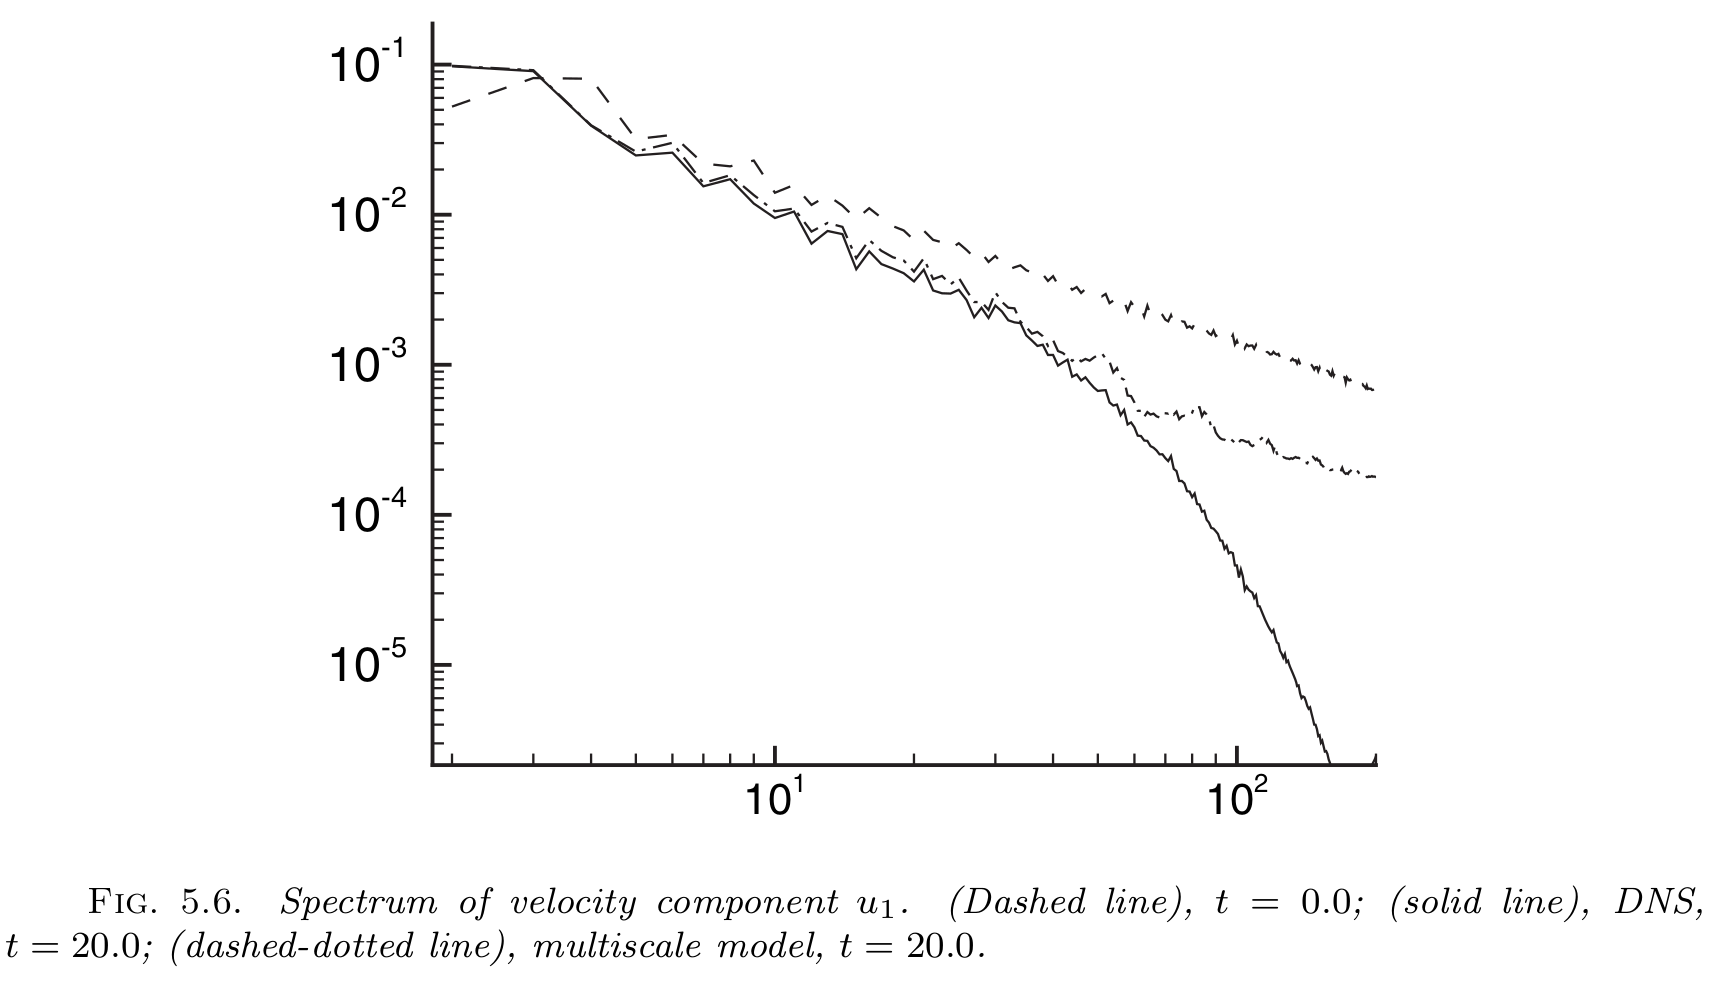
\includegraphics[width=1\linewidth]{Figures/spec2.png}
			
		\end{minipage}
	\end{figure}
\end{frame}

\begin{frame}[c]\frametitle{Innovations in Data assimilation}
	
\end{frame}

\begin{frame}[c]\frametitle{Algorithm}
	
\end{frame}

\begin{frame}[c]\frametitle{Result}
	
\end{frame}

%======================================================================

%======================================================================
\begin{frame}\frametitle{}

\vspace*{0.2in}

\begin{center}


\includegraphics[width=0.5\textwidth]{./template/smartAPI-logo-2.pdf}

\vspace*{0.35in}
\cPI{\huge Questions?}

\vspace*{0.5in}
\begin{minipage}{0.8\textwidth}
Thanks!!!!!!!!!!!!!
\end{minipage}

\end{center}


\end{frame}
%======================================================================



%======================================================================


\end{document}
